%%% Template originaly created by Karol Kozioł (mail@karol-koziol.net) and modified for ShareLaTeX use

\documentclass[a4paper,11pt]{article}

\usepackage[T1]{fontenc}
\usepackage[utf8]{inputenc}
\usepackage{graphicx}
\usepackage{xcolor}
\usepackage[]{authblk}
\usepackage{subcaption}
\usepackage{multirow}

\renewcommand\familydefault{\sfdefault}
\usepackage{tgheros}
\usepackage[defaultmono]{droidmono}

\usepackage{amsmath,amssymb,amsthm,textcomp}
\usepackage{enumerate}
\usepackage{multicol}
\usepackage{tikz}

\usepackage{geometry}
%\geometry{total={210mm,297mm},
%left=25mm,right=25mm,%
%bindingoffset=0mm, top=20mm,bottom=20mm}


\linespread{1.2}

\newcommand{\linia}{\rule{\linewidth}{0.5pt}}

% custom theorems if needed
\newtheoremstyle{mytheor}
    {1ex}{1ex}{\normalfont}{0pt}{\scshape}{.}{1ex}
    {{\thmname{#1 }}{\thmnumber{#2}}{\thmnote{ (#3)}}}

%\theoremstyle{mytheor}
%\newtheorem{defi}{Definition}

% my own titles
\makeatletter
\renewcommand{\maketitle}{
\begin{center}
\vspace{1ex}
{\LARGE \textsc{\@title}}
\vspace{0.5ex}
\linia\\
\@author \hfill \@date
%\@personNumber \hfill \@email
\vspace{3ex}
\end{center}
}
\makeatother
%%%

% custom footers and headers
\usepackage{fancyhdr}
\pagestyle{fancy}
\lhead{}
\chead{}
\rhead{}
\lfoot{HW 3}
\cfoot{}
\rfoot{Page \thepage}
\renewcommand{\headrulewidth}{0pt}
\renewcommand{\footrulewidth}{0pt}
%

% code listing settings
\usepackage{listings}
\lstset{
    language=Python,
    basicstyle=\ttfamily\small,
    aboveskip={1.0\baselineskip},
    belowskip={1.0\baselineskip},
    columns=fixed,
    extendedchars=true,
    breaklines=true,
    tabsize=4,
    prebreak=\raisebox{0ex}[0ex][0ex]{\ensuremath{\hookleftarrow}},
    frame=lines,
    showtabs=false,
    showspaces=false,
    showstringspaces=false,
    keywordstyle=\color[rgb]{0.627,0.126,0.941},
    commentstyle=\color[rgb]{0.133,0.545,0.133},
    stringstyle=\color[rgb]{01,0,0},
    numbers=left,
    numberstyle=\small,
    stepnumber=1,
    numbersep=10pt,
    captionpos=t,
    escapeinside={\%*}{*)}
}

%%%----------%%%----------%%%----------%%%----------%%%

\begin{document}

\title{Hw 3: Homography and fundamental matrix estimation}

\author{Avinash Kommineni, 50248877} 
%\personNumber{50248877}
%\email{akommineni@buffalo.edu}
%\personNumber {50248877}
%\email{akommineni@buffalo.edu}
\date{\today}

\maketitle

\section*{Output}

And the output images are as follows...\\
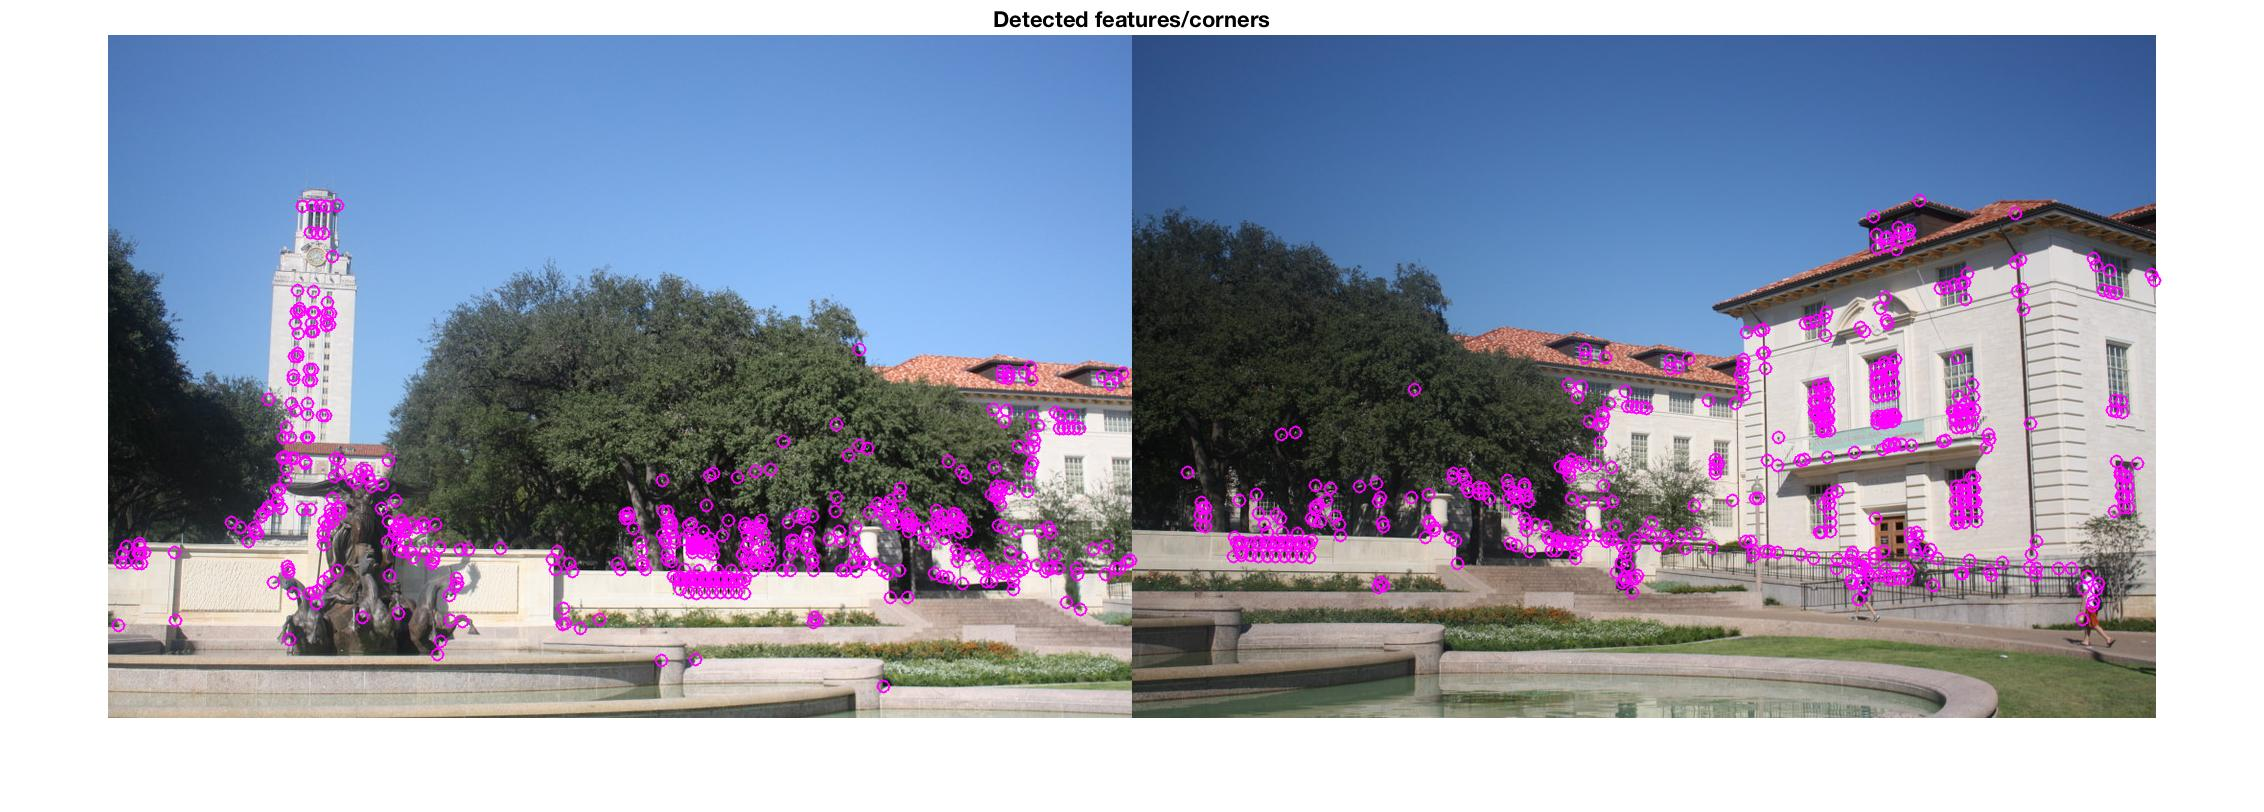
\includegraphics[width=\textwidth]{hw3/code/1}\\
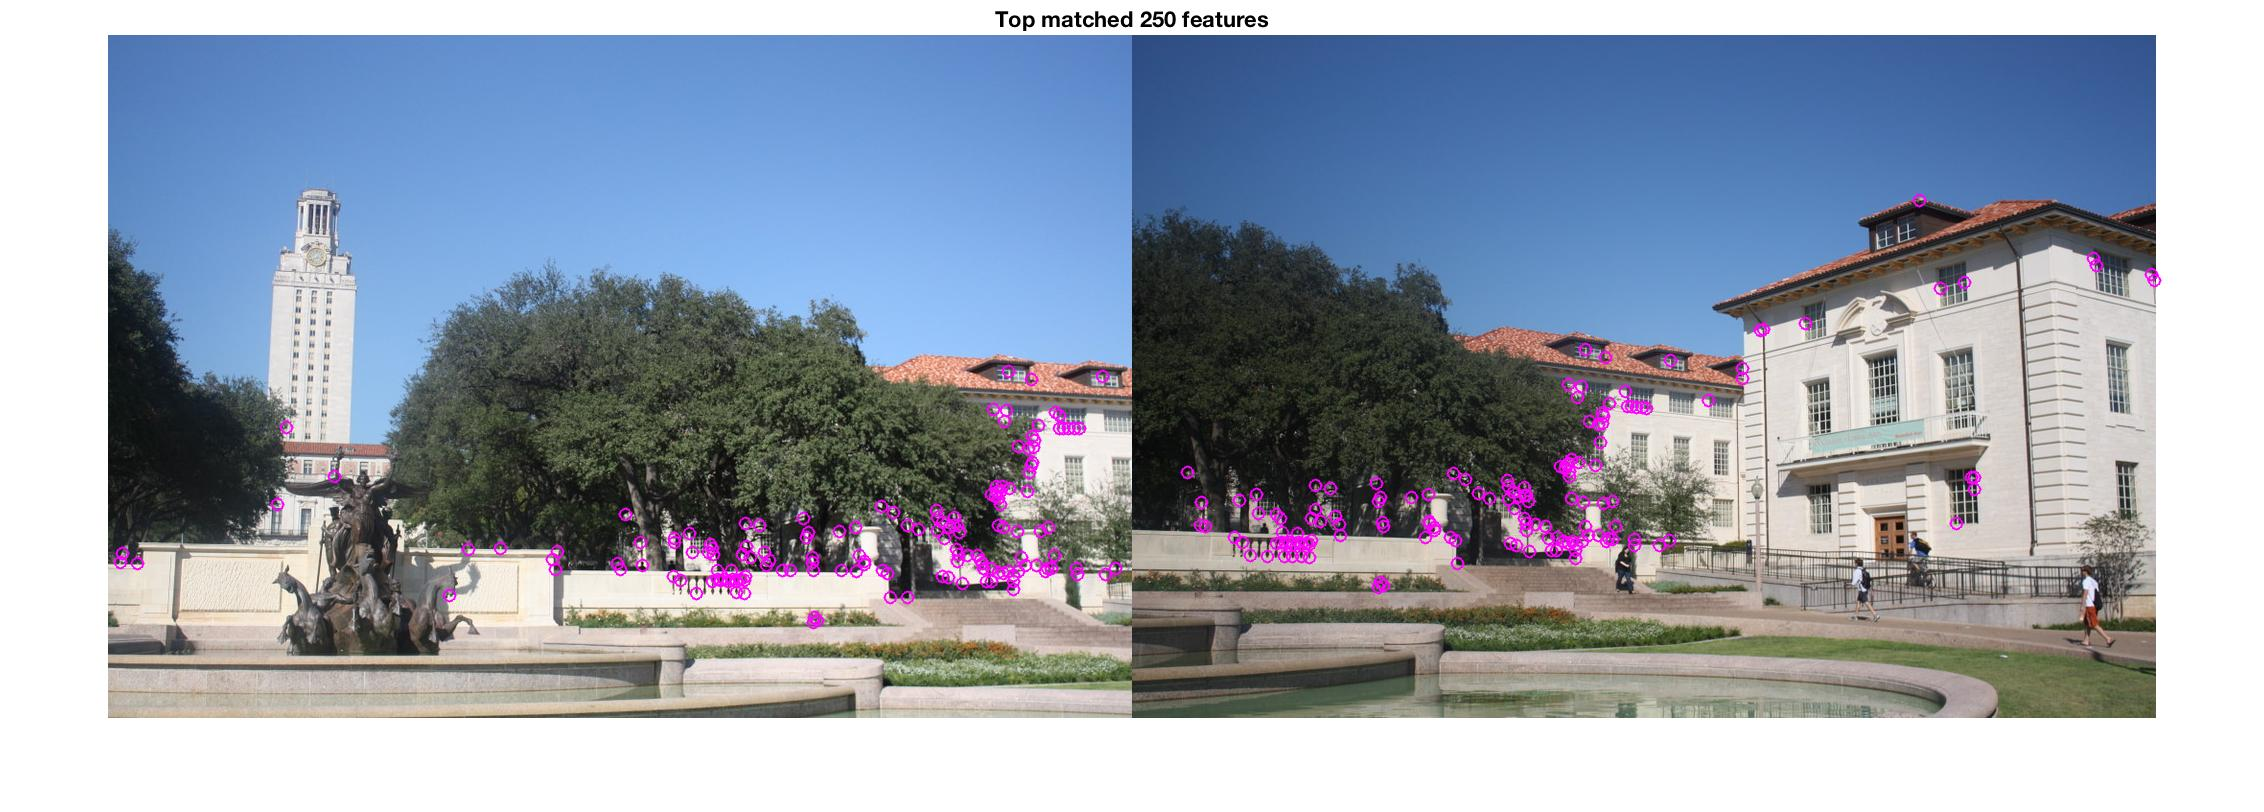
\includegraphics[width=\textwidth]{hw3/code/2}\\
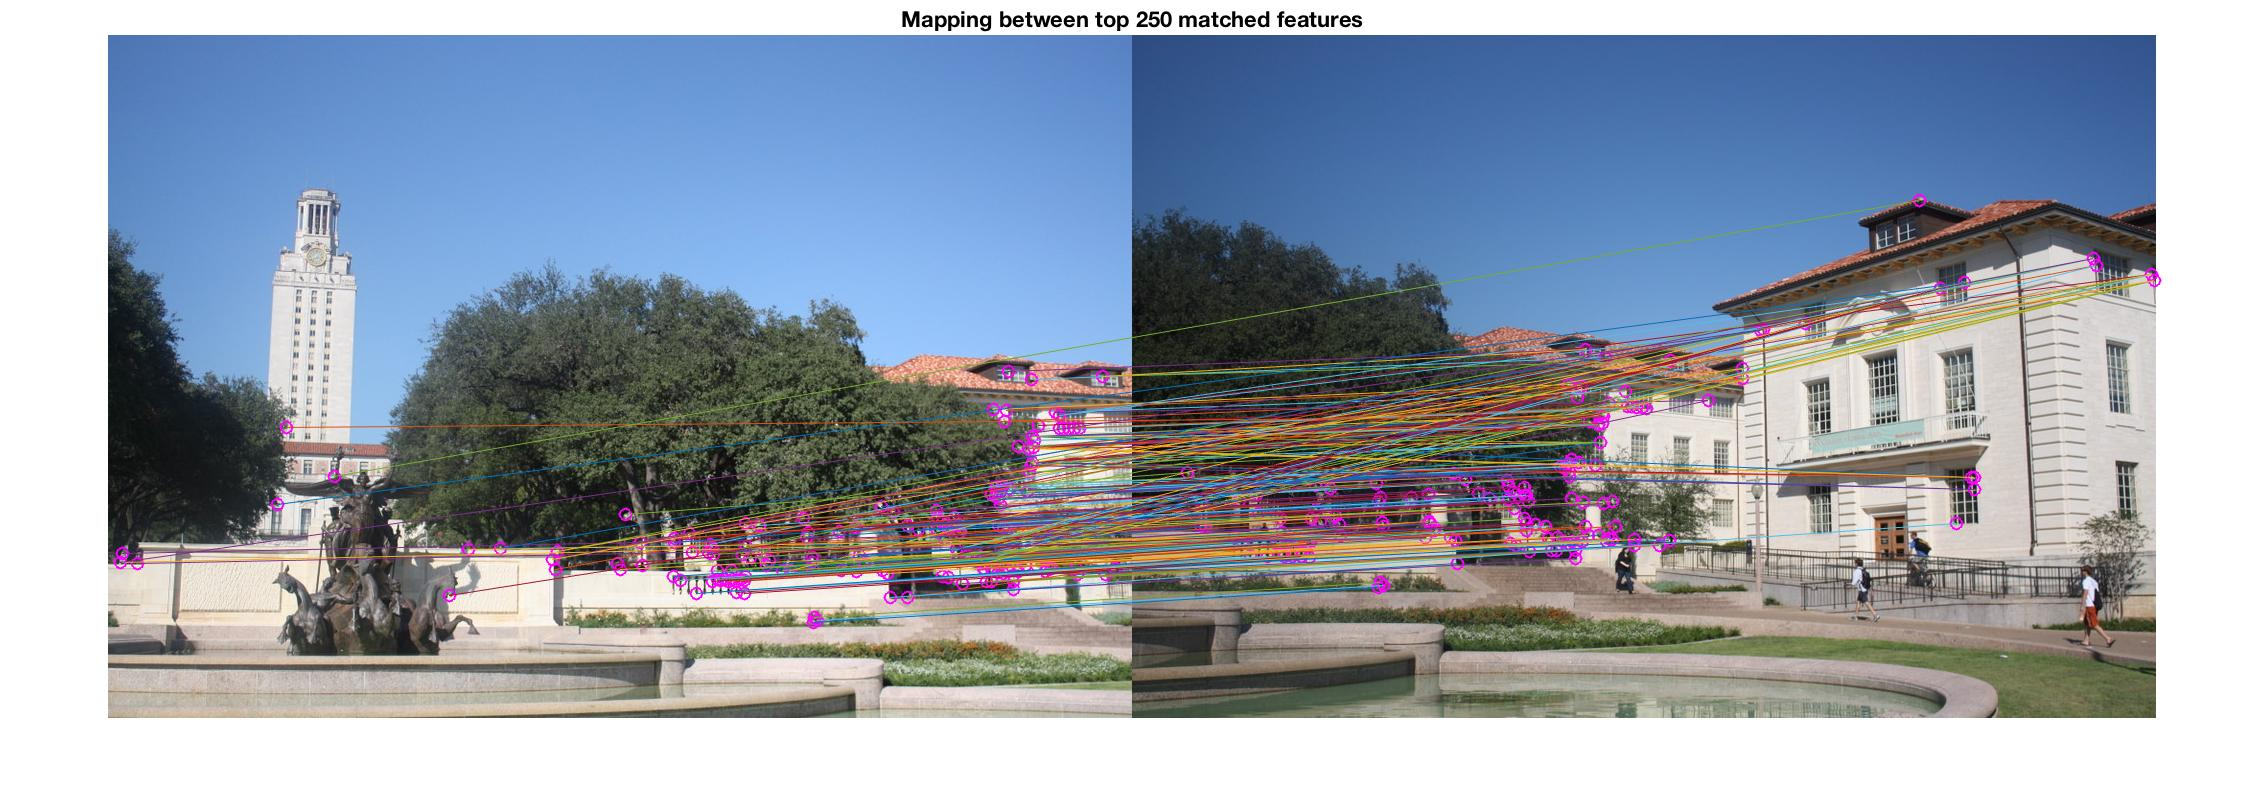
\includegraphics[width=\textwidth]{hw3/code/3}\\
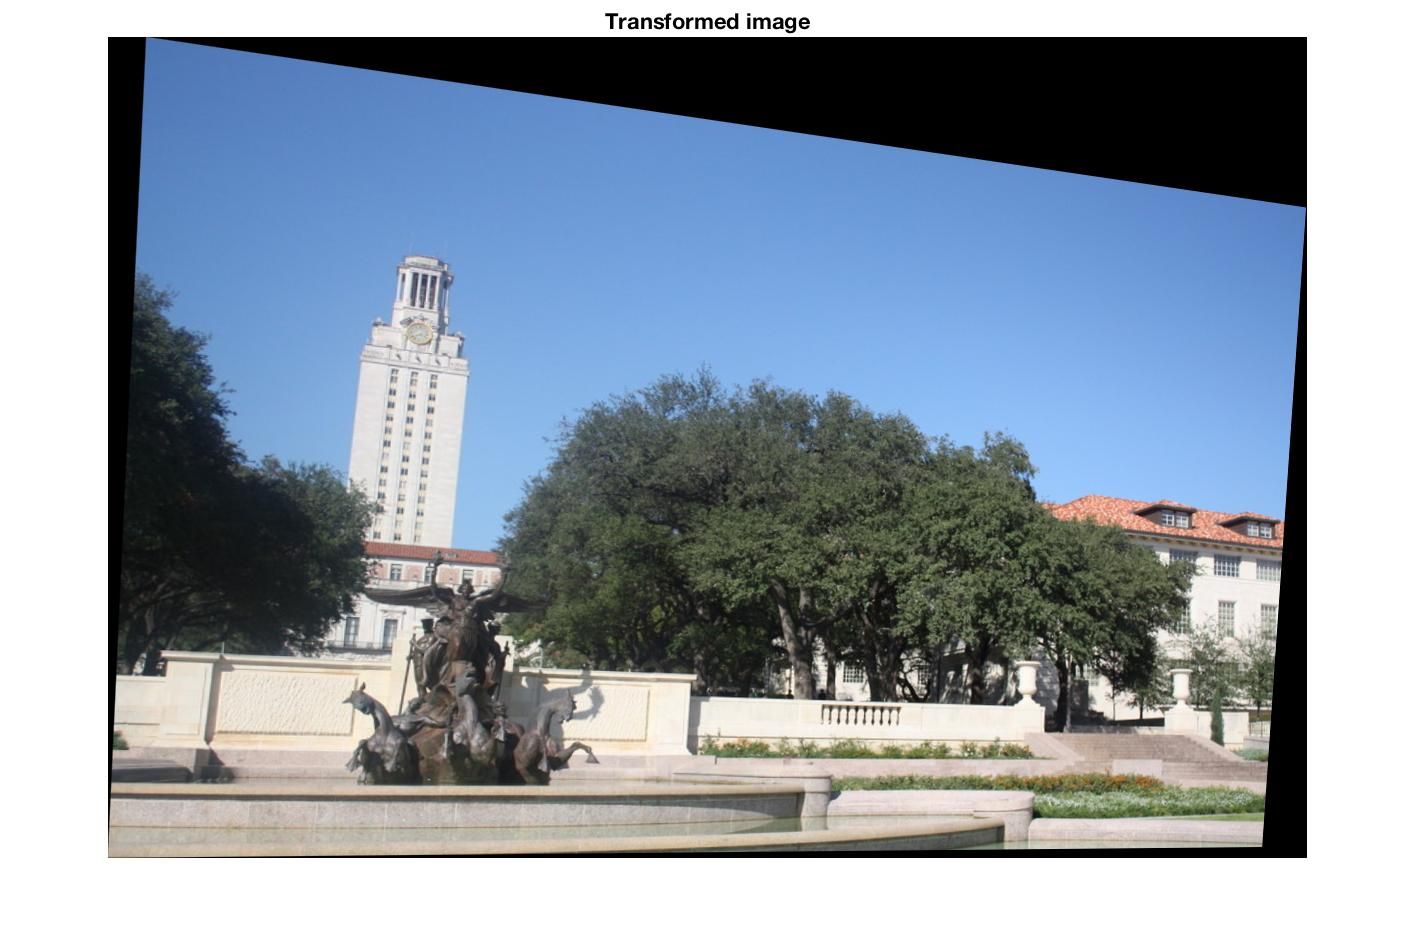
\includegraphics[width=\textwidth]{hw3/code/4}\\

Number of inliers: 129\\

Average: 1.4125\\
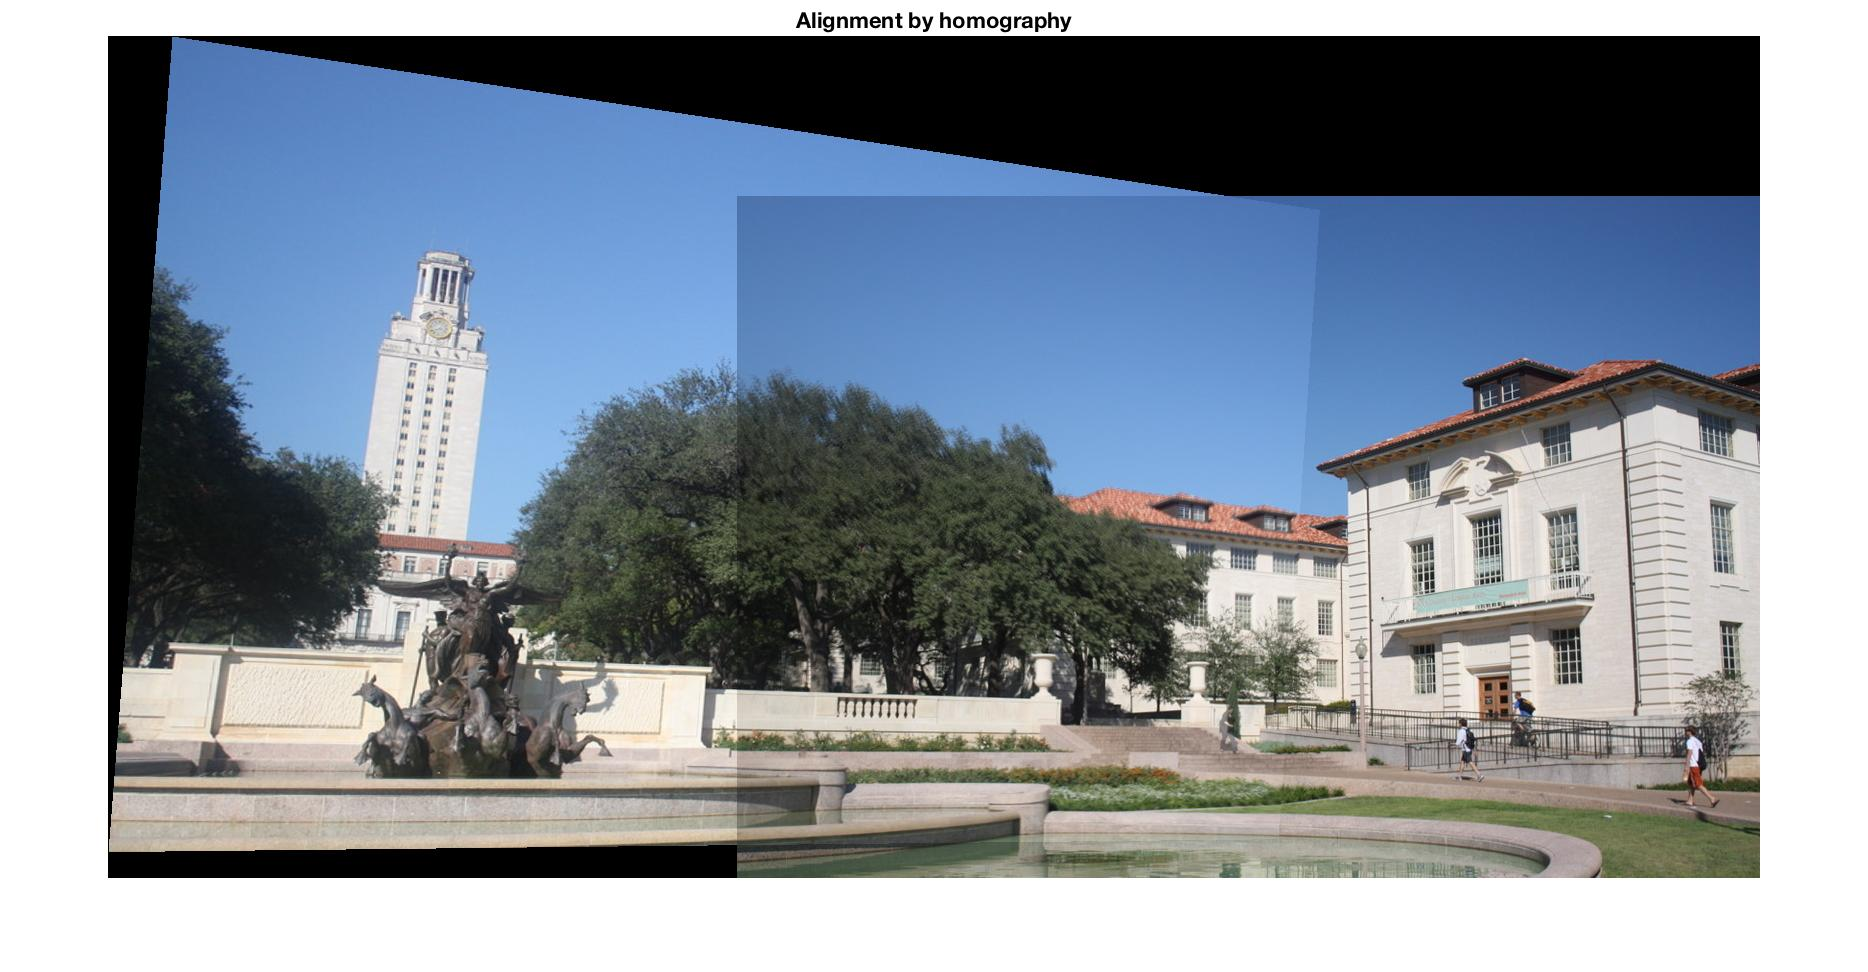
\includegraphics[width=\textwidth]{hw3/code/5}\\
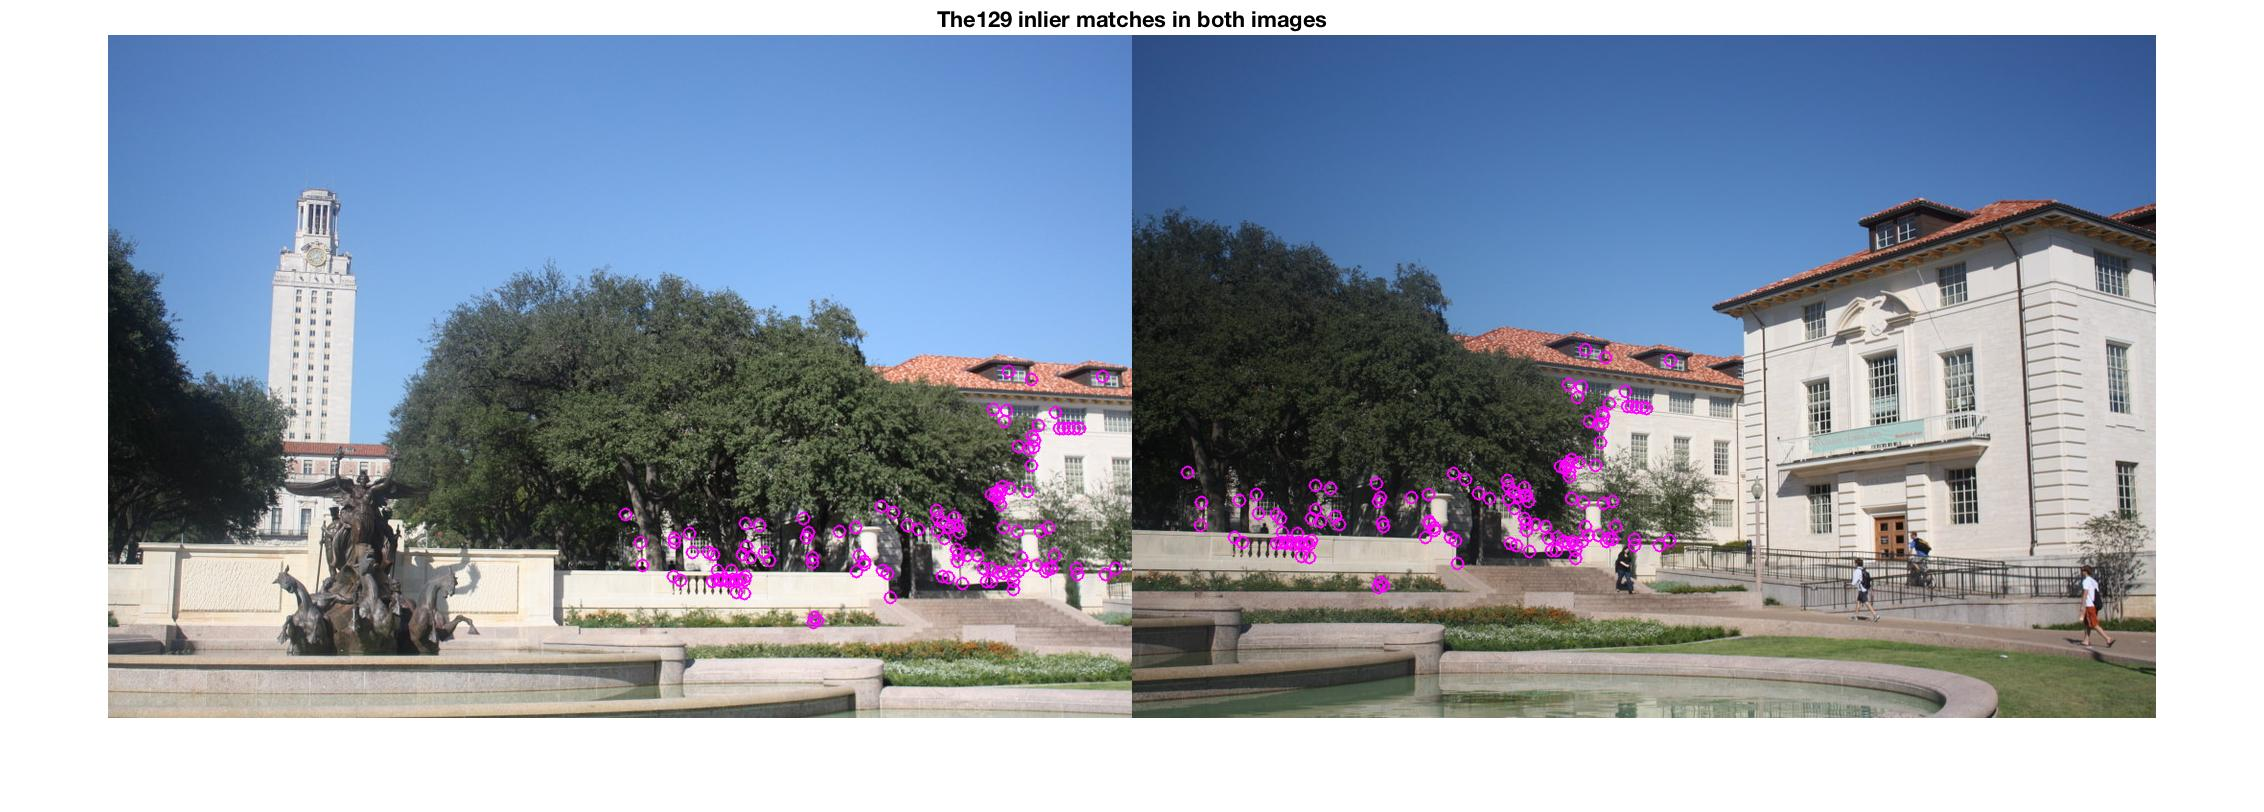
\includegraphics[width=\textwidth]{hw3/code/6}\\
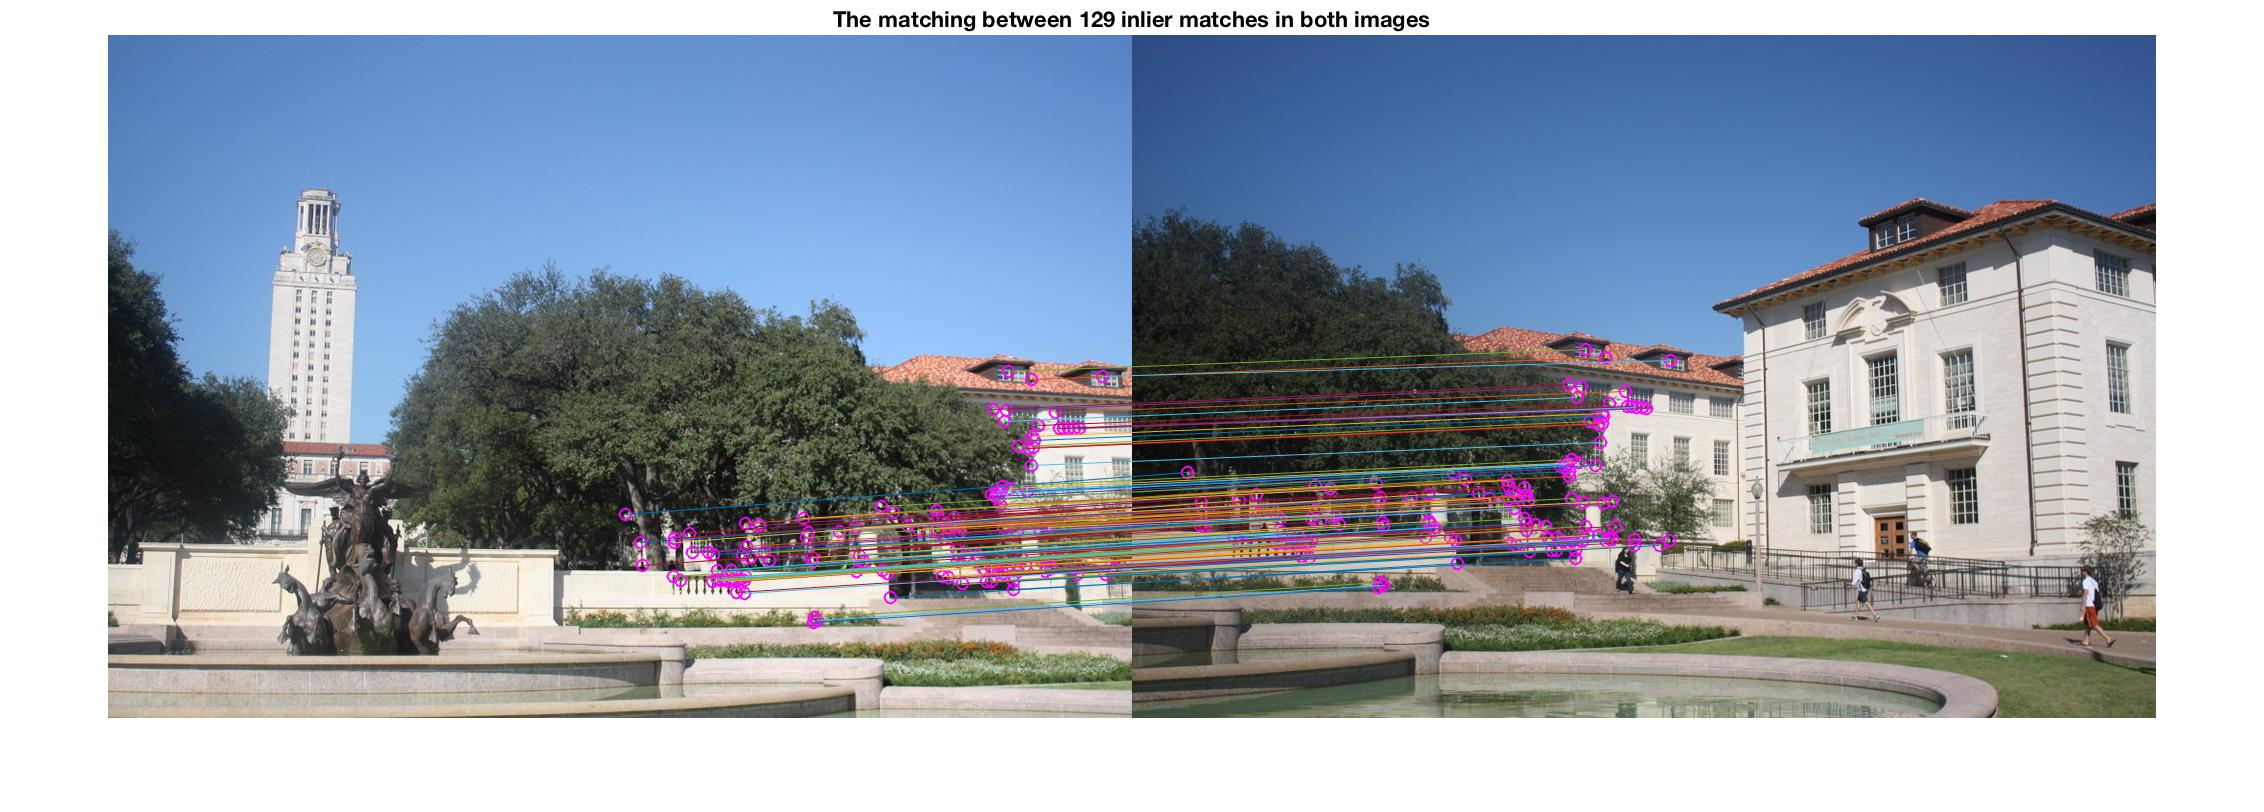
\includegraphics[width=\textwidth]{hw3/code/7}\\
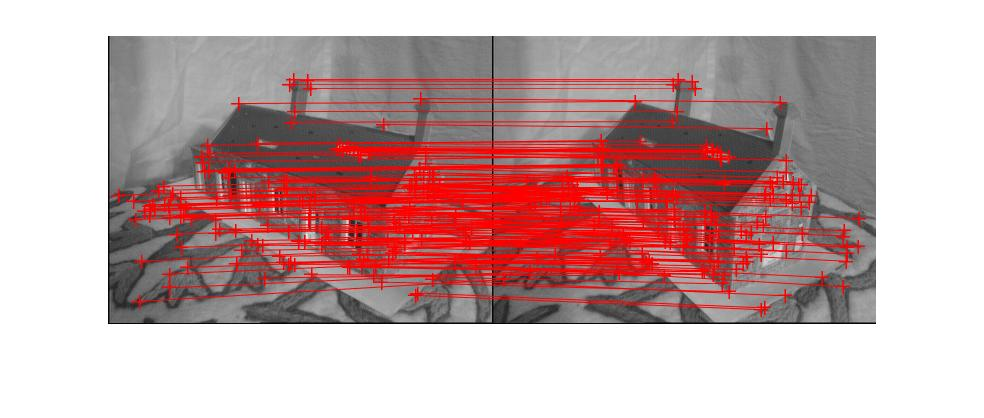
\includegraphics[width=\textwidth]{hw3/data/part2/1}\\

Normalised\\
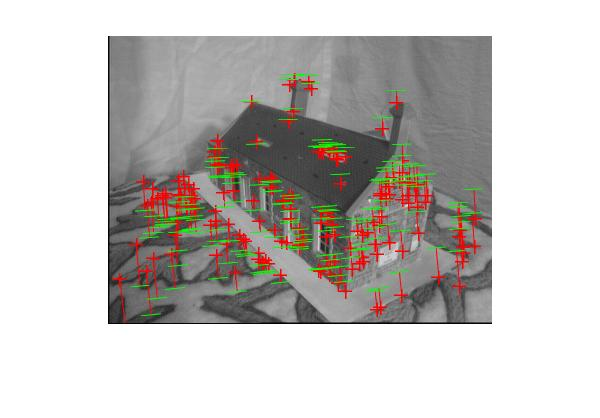
\includegraphics[width=\textwidth]{hw3/data/part2/2}\\
\vfill
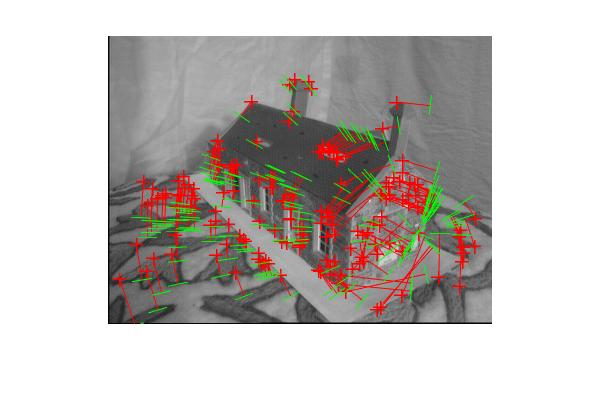
\includegraphics[width=\textwidth]{hw3/data/part2/2_2}
Un-normalised\\
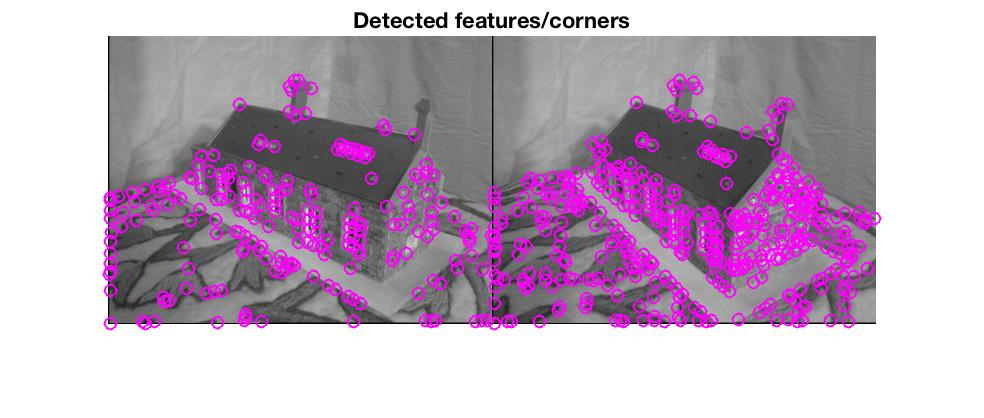
\includegraphics[width=\textwidth]{hw3/data/part2/4_1}\\
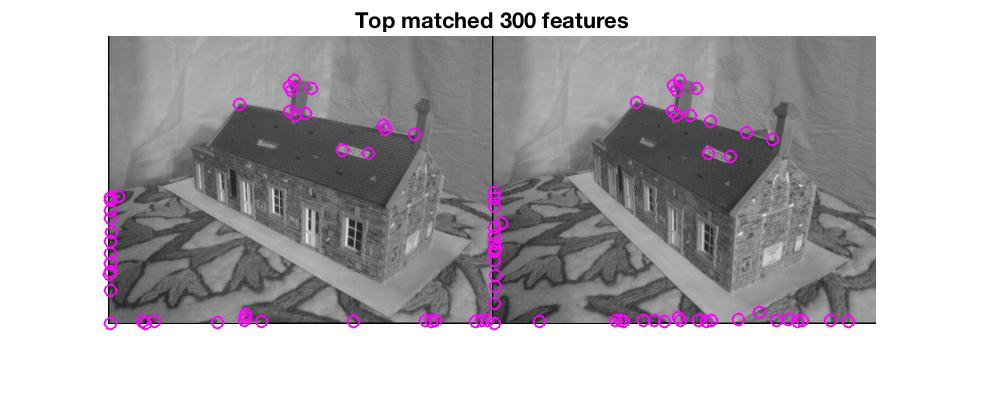
\includegraphics[width=\textwidth]{hw3/data/part2/4_2}\\
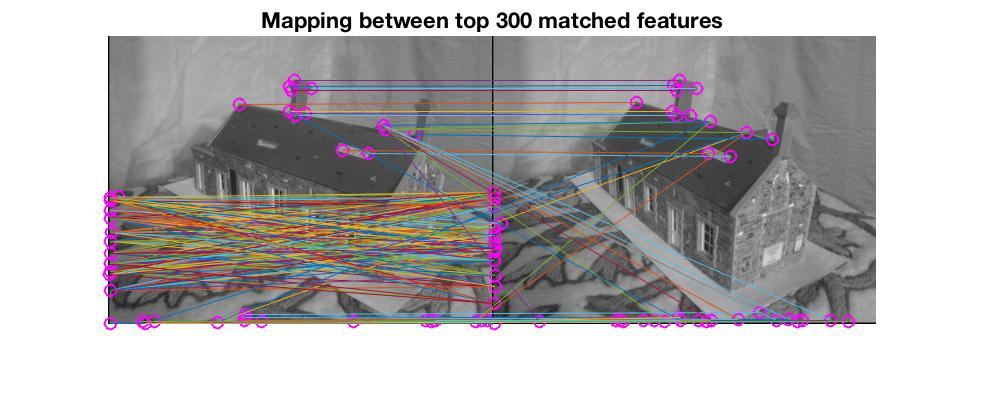
\includegraphics[width=\textwidth]{hw3/data/part2/4_3}\\


Number of inliers: 111\\

Average: 3.0563\\
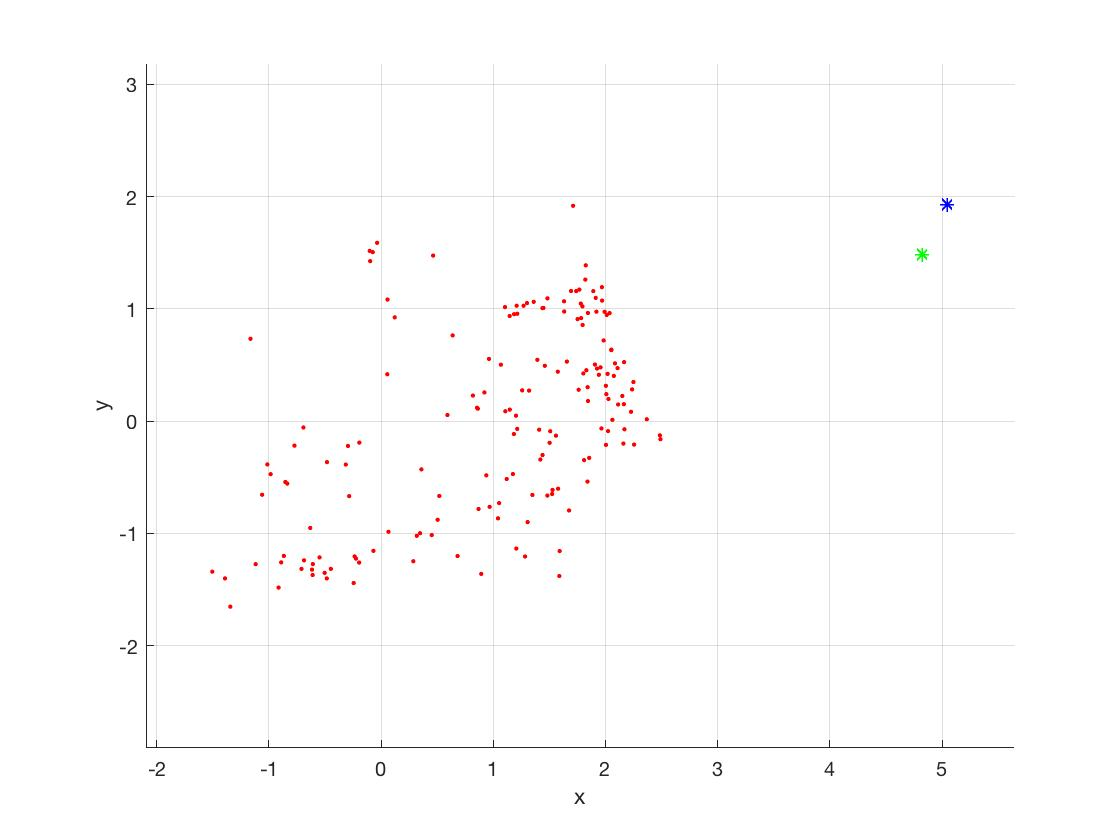
\includegraphics[width=\textwidth]{hw3/data/part2/5}\\
\vfill

%\section*{Effecient vs Inefficient}
%
%\begin{center}
%	\begin{tabular}{ |c|c|c|c| } 
%		\hline
%		Time taken (sec) & Image Downscaling & Filter Up-scaling \\
%		\hline
%		\multirow{8}{7em}{Image run time for the given 4 images and custom 4 images} & 0.063426 & 0.326780 \\ 
%		& 0.122941 & 0.502245  \\ 
%		& 0.075058 & 0.312024 \\ 
%		& 0.055799 & 0.230015 \\ 
%		& 1.524554 & 12.276676 \\ 
%		& 0.471535 & 3.284120 \\ 
%		& 0.180295 & 1.275178 \\
%		& 0.327218 & 2.362955 \\
%		\hline
%	\end{tabular}
%\end{center}
%
%\section*{Notes}
%\begin{itemize}
%	\item The time increases rapidly for the case of filter up-scaling and especially for the for those custom images which are bigger in size.
%	\item The time increases for the case of sigma$(\sigma)$=2.0. It increases significantly for the filter up-scaling and marginally for the other one.
%	\item 	\begin{tabular}{ |c|c|c|c| } 
%		\hline
%		Time taken (sec) & Image Downscaling & Filter Up-scaling \\
%		\hline
%		\multirow{8}{7em}{Image run time for the given 4 images and custom 4 images} & 0.065452 & 0.759418 \\ 
%		& 0.096532 & 0.925315  \\ 
%		& 0.062356 & 0.580354 \\ 
%		& 0.075324 & 0.431651 \\ 
%		& 1.474615 & 23.838904 \\ 
%		& 0.446366 & 5.750504 \\ 
%		& 0.172011 & 2.333773 \\
%		& 0.328813 & 3.933201 \\
%		\hline
%	\end{tabular}
%	\vfill
%	
%	\item The same image with sigma as 1.4 and 2.0\\
%%	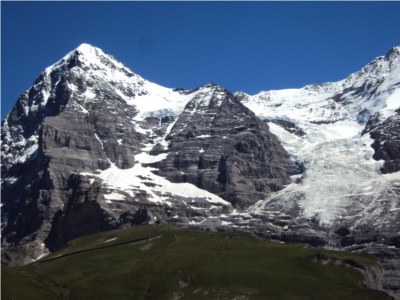
\includegraphics[scale=0.25]{hw2/code/1}\\
%%	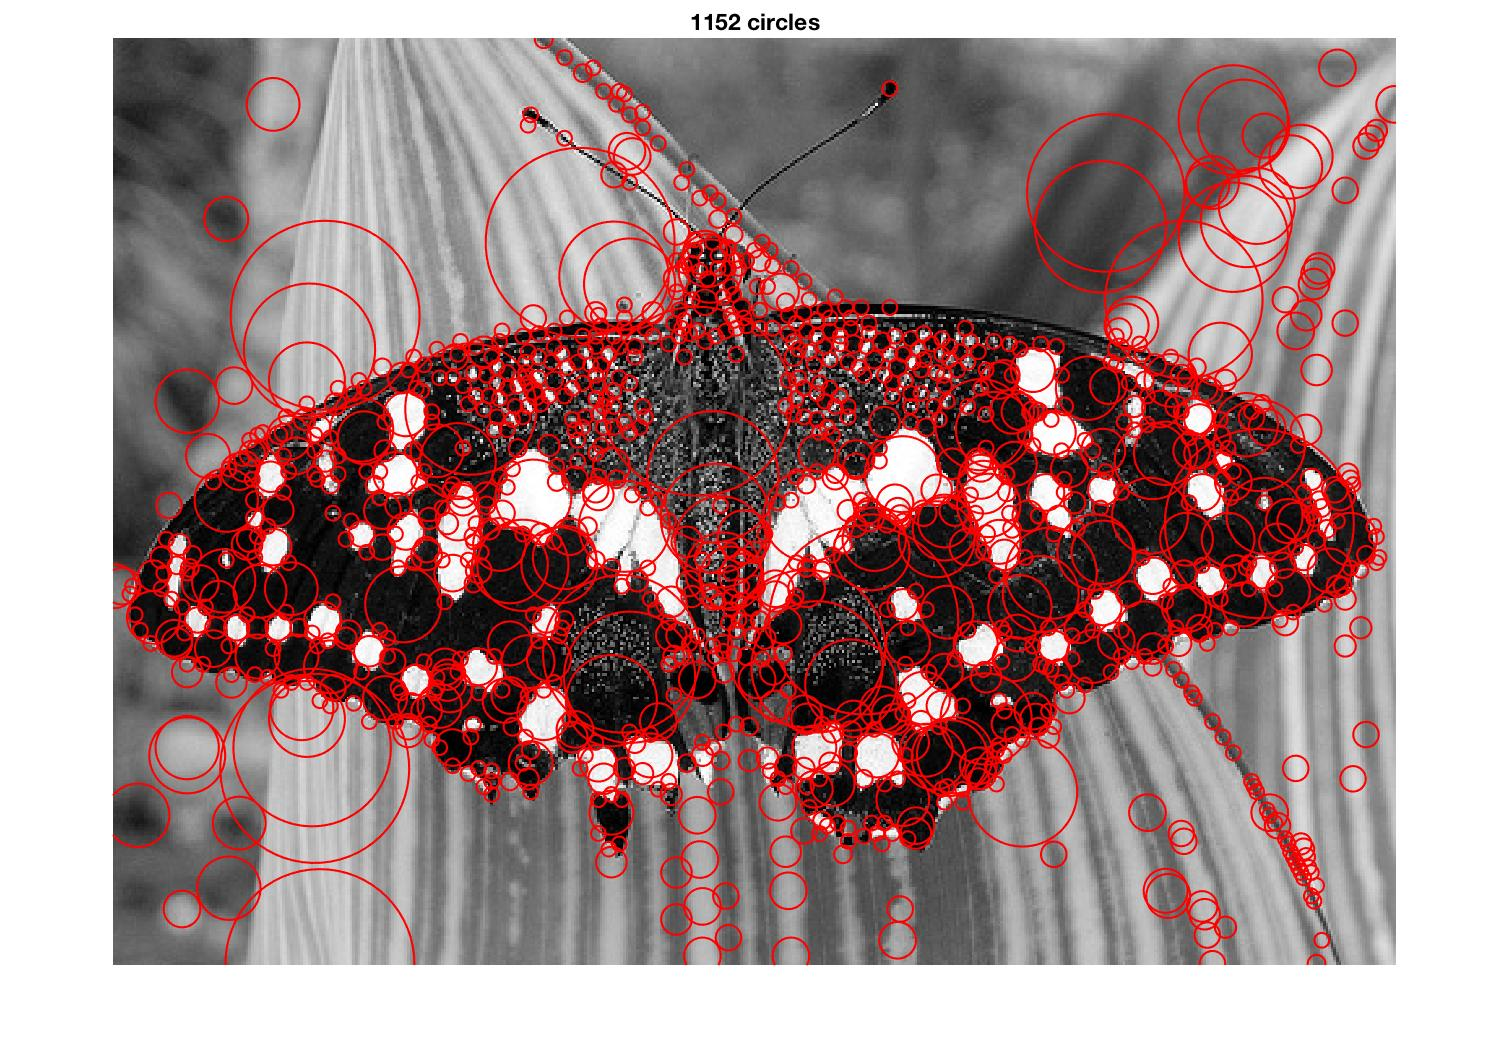
\includegraphics[scale=0.25]{hw2/code/1_1}\\
%	Not much differences between two except that the first image has got granular part covered because it's sigma is low.
%	\item Thick and sharp edges like the text in $5^{th}$ image is picked up every layer of the filter so the thick resultant circles.
%	\item The images produced with filter up-scaling are found in the folder FilterScaled.
%	\item While implementing the 3D nonmaximum suppression, the border condition was handled by replicating the first and layer of scale space layers.
%	\item Deponding upon the value of sigma, the value of threshold must also be adjusted so that the image is not too over or scarcely populated with circles.
%	
%\end{itemize}
\end{document}
